\secnumbersection{PROPUESTA DE SOLUCIÓN}

Se debe desarrollar la solución propuesta. Los subcapítulos por poner aquí son propios del autor. Se sugiere mencionar metodología usada. Es conveniente incorporar figuras y tablas para aclarar la solución, que deben indicar el número de la figura, su nombre y su autor o fuente (si las diseñas tú, la fuente es ``Elaboración propia''). Ver ejemplos en esta página y en la siguiente.

Cabe mencionar que aquí está la esencia del trabajo en lo que se refiere al aporte creativo del memorista, es el momento de demostrar que usted es un destacado profesional que creó, diseñó y/o llevó a cabo la solución propuesta.

\subsection{EJEMPLO DE COMO CITAR FIGURAS E ILUSTRACIONES}

Se colocó una imagen que se puede referenciar también desde el texto (Ver figura \ref{fig:malla}).

\begin{figure}[h]
\centering
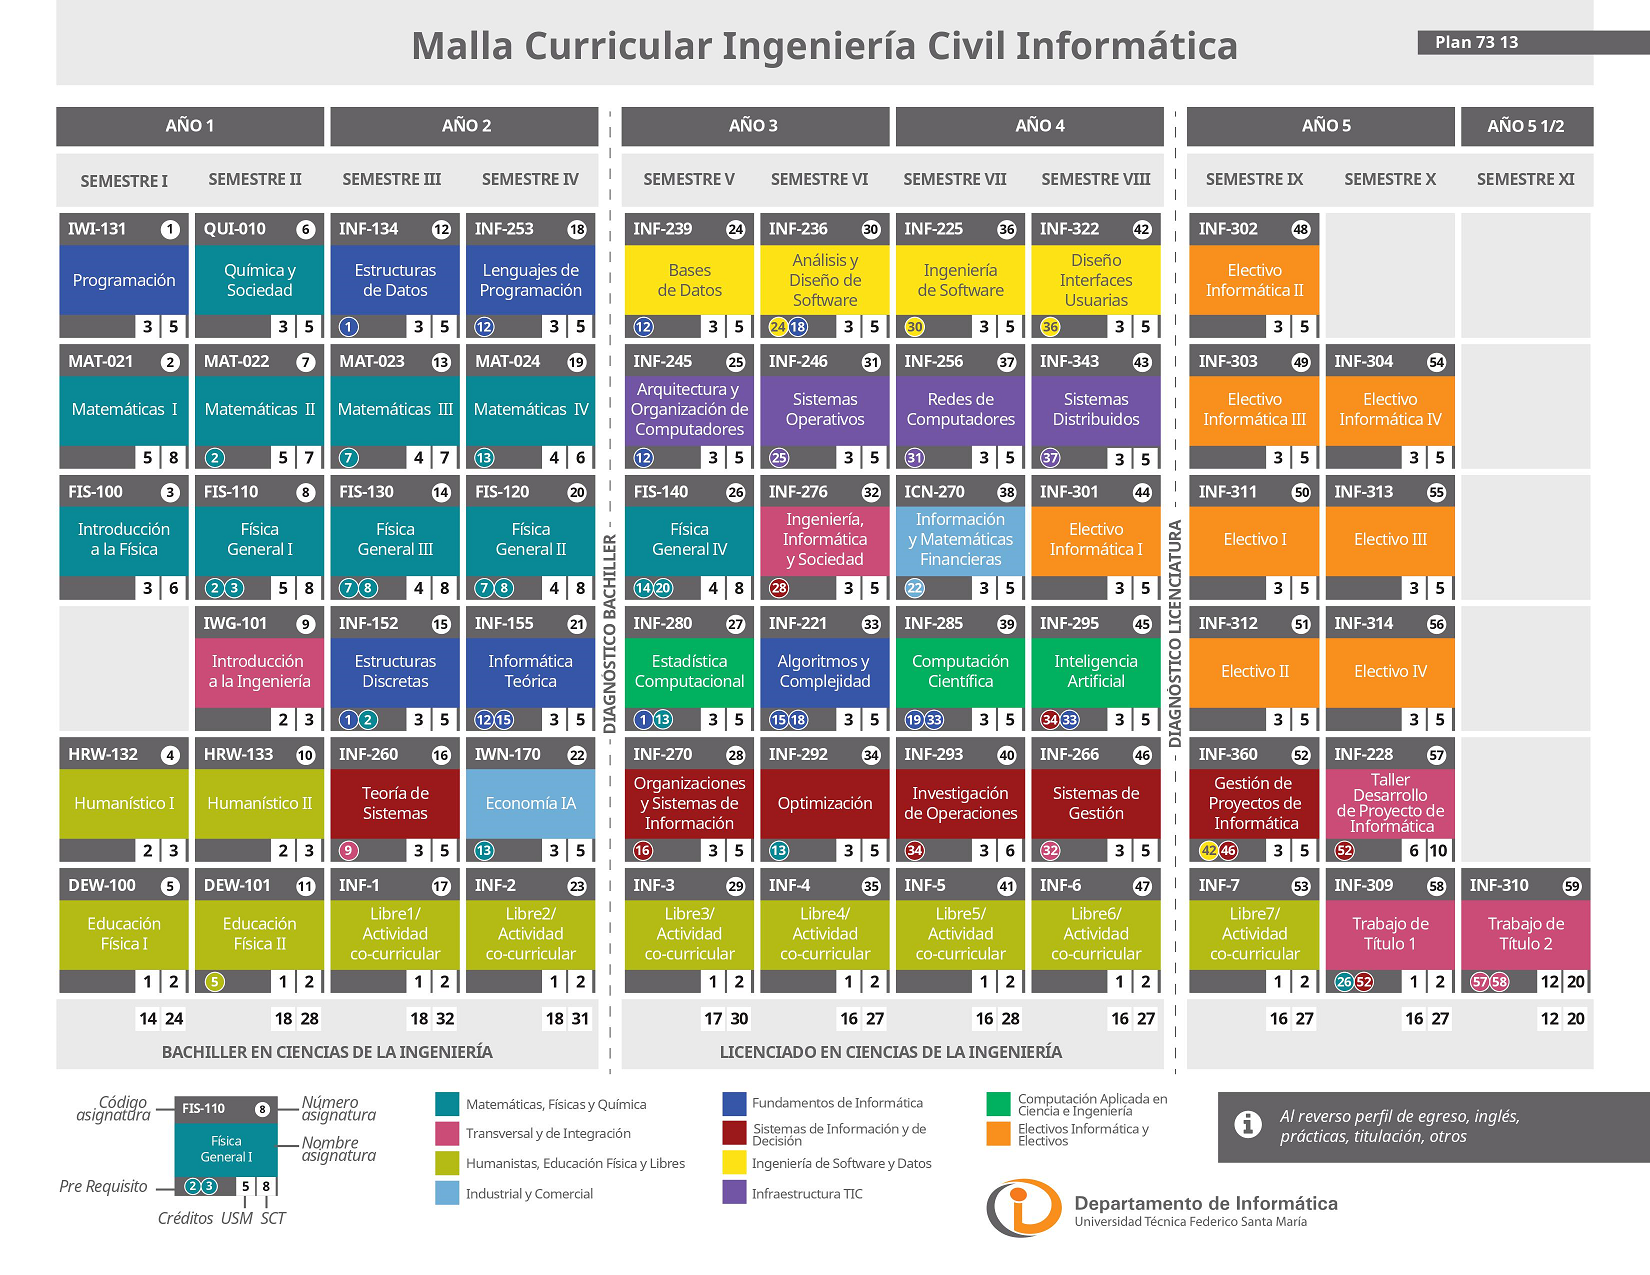
\includegraphics[width=0.8\textwidth]{malla_ingenieria_informatica}
\caption{\label{fig:malla} Malla Curricular Ingeniería Civil Informática.} Fuente: Departamento de Informática.
\end{figure}
